% !TEX root = ../../../main.tex
% 来源：中学数学实验教材·第三册（高中数学）
% 章节：三角函数的图象和性质 / 余弦函数的图象和性质
% 原始文件：7.tex，行 541-570
% 类型：tikz
% ---
     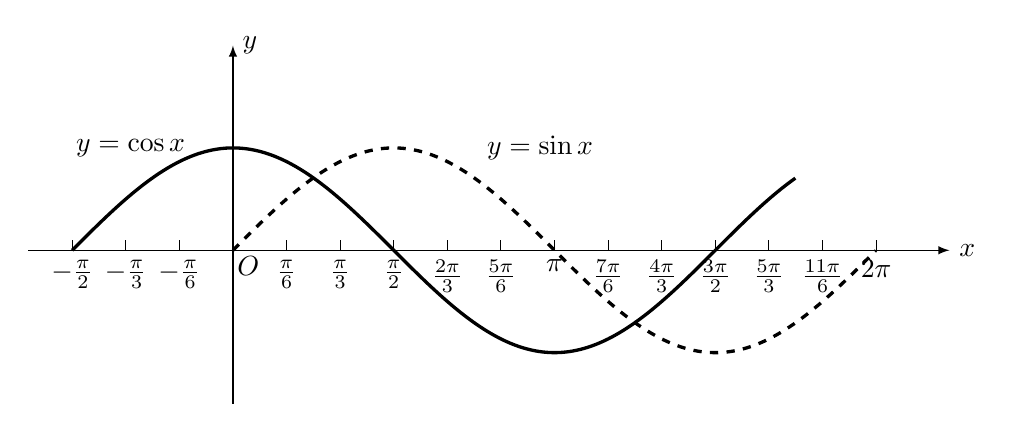
\begin{tikzpicture}[scale=1.3, >=latex]

\draw[->] (-2,0)--(7,0)node[right]{$x$};
\draw [->](0,-1.5)--(0,2)node[right]{$y$};
\draw[domain=0 : pi*2,  samples=1000, very thick, dashed] plot(\x, {sin(\x r)});
\draw[domain=-0.5*pi : pi*1.75,  samples=1000, very thick] plot(\x, {cos(\x r)});

\foreach \x in {-3,-2,...,12}
{
    \draw (\x*pi/6, 0)--(\x*pi/6, .1);
}
\node at (-1,1){$y=\cos x$};  \node at (3,1){$y=\sin x$};

\node at (-3*pi/6, 0)[below]{$-\frac{\pi}{2}$};
\node at (-2*pi/6, 0)[below]{$-\frac{\pi}{3}$};
\node at (-1*pi/6, 0)[below]{$-\frac{\pi}{6}$};
\node at (1*pi/6, 0)[below]{$\frac{\pi}{6}$};
\node at (2*pi/6, 0)[below]{$\frac{\pi}{3}$};
\node at (3*pi/6, 0)[below]{$\frac{\pi}{2}$};
\node at (4*pi/6, 0)[below]{$\frac{2\pi}{3}$};
\node at (5*pi/6, 0)[below]{$\frac{5\pi}{6}$};
\node at (6*pi/6, 0)[below]{$\pi$};
\node at (7*pi/6, 0)[below]{$\frac{7\pi}{6}$};
\node at (8*pi/6, 0)[below]{$\frac{4\pi}{3}$};
\node at (9*pi/6, 0)[below]{$\frac{3\pi}{2}$};
\node at (10*pi/6, 0)[below]{$\frac{5\pi}{3}$};
\node at (11*pi/6, 0)[below]{$\frac{11\pi}{6}$};
\node at (12*pi/6, 0)[below]{$2\pi$};
\node at (.15,-.15){$O$};
     \end{tikzpicture}
